
\chapter{Week4}

\section{Friday}\index{week4_Friday_lecture}
\subsection{Linear Transformation}
Start with a matrix $\bm A$. When multiplying $\bm A$ with a vector $\bm v$, it transform $\bm v$ to another vector $\bm{Av}$. Matrix multiplication $L(\bm v) = \bm{Av}$ gives a \emph{linear transformation}:
\begin{definition}[linear transformation]
A transformation $L$ assigns an output $T(\bm v)$ to each inpout vector $\bm v$ in $\bm V$.\\
The transformation is \emph{linear transformation} if it satisfies
\[
L(\alpha \bm v_1 + \beta \bm v_2)=\alpha L(\bm v_1)+\beta L(\bm v_2)
\]
for all vector $v_1,v_2$ and scalar $\alpha,\beta$.
\end{definition}
\emph{Key Observation:} If the input is $\bm v = \bm 0$, the output must be $L(\bm v) = \bm 0$.
\subsubsection{The idea of linear transformation}
Given linear transformation $L: \mathbb{R}^{n}\mapsto\mathbb{R}^{m}$, let's show that in order to study the output we only need to start from the \emph{basis} of our output: \\
\enlargethispage{1cm}
Assume the basis of $\mathbb{R}^{n}$ is $\{e_1,e_2,\dots,e_n\}$, where $L(e_i)=a_i\in\mathbb{R}^{m}$ for $i=1,\dots,n$.\\
Notice that \emph{The rule of linearity extends to combinations of three vectors or $\bm n$ vectors.}\\
Hence given any vector $\bm x=x_1e_1+x_2e_2+\dots+x_ne_n\in\mathbb{R}^{n}$, we express its transformation in matrix multiplication form:
\[
\begin{aligned}
L(\bm x) &= L(x_1e_1+x_2e_2+\dots+x_ne_n)\\
			 &= x_1L(e_1)+x_2L(e_2)+\dots+x_nL(e_n)\\
			 &= x_1a_1+x_2a_2+\dots+x_na_n=\begin{bmatrix}
a_1&a_2&\dots&a_n
\end{bmatrix}\begin{bmatrix}
x_1\\x_2\\\dots\\x_n
\end{bmatrix}\\
			 &= \bm{Ax}
\end{aligned}
\]
where $\bm A$ is a $m\x n$ matrix with columns $a_1,\dots,a_n$.\newpage

\subsubsection{Matrix defines linear transformation}
Conversely, given $m\x n$ matrix $\bm A$, $L(\bm x) = \bm{Ax}$ defines a linear mapping. This is because matrix multiplication is also a lienar operator.\\
\begin{remark}
Transformations have a new ``language''. For example, for nonlinear transformation, if there is \emph{no matrix}, we cannot talk about a \emph{column space}. But this idea could be rescued. We know the \textit{column space} consists of all outputs $\bm{Av}$, the \textit{nullspace} consists of all inputs for which $\bm{Av}=\bm 0$. We could translate those terms into ``range'' and ``kernel'':
\end{remark}
\begin{definition}[range]
For a linear transformation $L:V\mapsto W$, the range (or image) of $L$ refers to the set of all outputs $T(\bm v)$, which is denoted as:
\[
\Range(L)=\{L(\bm x):x\in\bm V\}
\]
Sometimes we also use notation $\im(L)$ to express the same thing.
\end{definition}
\emph{The range corresponds to column space}. If $L(\bm x)=\bm{Ax}$, we have $\Range(L)=\col(\bm A)$.
\begin{definition}[kernel]
The kernel of $L$ refers to the set of all inputs for which $L(\bm v)=\bm 0$, which is denoted as:
\[
\ker(L)=\{\bm x:L(\bm x)=\bm 0\}
\]
\end{definition}
\emph{Kernel corresponds to nullspace}. If $L(\bm x)=\bm{Ax}$, we have $\ker(L)=N(\bm A)$.
\begin{remark}
For linear transformation $L:\bm V\mapsto \bm W$, where $L(\bm x)=\bm{Ax}$. We have two rules:
\[
\begin{aligned}
N(\bm A)&\mapsto \{\bm 0\}\\
\bm V&\mapsto \col(\bm A)
\end{aligned}
\]
\end{remark}
\subsection{Example: differentiation}
\emph{Key idea of this section:}\\
\hspace*{1cm}{\bfseries\textit{Suppose we know $L(\bm v_1),\dots,L(\bm v_n)$ for the basis vectors $\bm v_1,\dots,\bm v_n$,Then the linearity produces $L(\bm v)$ for every other input vector $\bm v$.}}\\
\emph{Reason:} Every $\bm v$ is a unique combination $c_1\bm v_1+\dots+c_n\bm v_n$ of the basis vector $\bm v_i$. Suppose $L$ is a linear transformation, $L(\bm v)$ must be the \emph{same combination} $c_1L(\bm v_1)+\dots+c_nL(v_n)$ of the \emph{known outputs} $L(\bm v_i)$.\\\\
The derivative of the functions $1,x,x^2,x^3$ are $0,1,2x,3x^2$. If we consider ``\emph{taking the derivative}'' as a transformation, whose inputs and outputs are functions, then we claim that the \emph{derivative transformation} is \emph{linear}:
\[
L(\bm v)=\frac{\diff \bm v}{\diff x}\qquad\text{obeys the linearity rule}\qquad\frac{\diff}{\diff x}(c\bm v+d\bm w) = c\frac{\diff \bm v}{\diff x}+d\frac{\diff \bm w}{\diff x}
\]
If we consider $1,x,x^2,x^3$ as vectors instead of functions, we notice they form a basis for the space $\bm V$ of \textit{polynomials with degree$\le 3$}. Find derivatives of these four basis tells us all derivatives in $\bm V$:
\begin{example}
Given any vector $\bm v$ in $\bm V$, it can be expressed as $\bm v=a+bx+cx^2+dx^3$. Thus we want to find the derivative transformation output for $\bm v$:
\[
\begin{aligned}
L(\bm v)&=aL(1)+bL(x)+cL(x^2)+dL(x^3)\\
        &=a\x(0)+b\x(1)+c\x(2x)+d\x(3x^2)\\
        &=b+2cx+3dx^2
\end{aligned}
\]
Can we express this linear transformation $L$ by a matrix $\bm A$? The answer is \textit{Yes}:\\
The derivative transforms the space $\bm V$ of cubics to the space $\bm W$ of quadratics. The basis for $\bm V$ is $1,x,x^2,x^3$. The basis for $\bm W$ is $1,x,x^2$. \textit{The derivative matrix is 3 by 4}:
\[
\bm A= \begin{bmatrix}
0&1&0&0\\0&0&2&0\\0&0&0&3
\end{bmatrix}=\text{\emph{matrix form of derivative $L$}}.
\]
Why is $\bm A$ the correct matrix? Because \emph{multiplying by $\bm A$ agrees with transforming by $L$}. The derivative of $\bm v=a+bx+cx^2+dx^3$ is $L(\bm v)=b+2cx+3dx^2$. The same numbers $b$ and $2c$ and $3d$ appear when we multiply by matrix $\bm A$:
\[
\textit{\emph{Take the derivative}}\qquad
\begin{bmatrix}
0&1&0&0\\0&0&2&0\\0&0&0&3
\end{bmatrix}\begin{bmatrix}
a\\b\\c\\d
\end{bmatrix}=\begin{bmatrix}
b\\2c\\3d
\end{bmatrix}.
\]
What does the matrix $\begin{bmatrix}
a\\b\\c\\d
\end{bmatrix}$ and $\begin{bmatrix}
b\\2c\\3d
\end{bmatrix}$ mean? \\It is the \emph{coordinate vector} of $\bm v$ and $L(\bm v)$. If we consider $a+bx+cx^2+dx^3$ as a vector, then it's better for us to study its coordinate vector $\begin{bmatrix}
a\\b\\c\\d
\end{bmatrix}$.\\ Hence taking derivative of $\bm v$ is the same as multiplying matrix $\bm A$ by its coordinate vector.
\end{example}



\subsubsection{The inverse of the derivative.}
The \emph{integral} is the inverse of the derivative. That is the Fundamental Theorem of Calculus. We see it now in linear Algebra. The integral transformation $L^{-1}$ that \textit{takes the integral from 0 to x} is linear! Applying $L^{-1}$ to $1,x,x^2$, which are $\bm w_1,\bm w_2,\bm w_3$:
\[
\text{\emph{Integration is $L^{-1}$}}\qquad
\int_0^x1\diff x=x,\quad\int_0^xx\diff x=\frac{1}{2}x^2,\quad\int_0^xx^2\diff x=\frac{1}{3}x^3.
\]
By linearity, the integral of $\bm w=B+Cx+Dx^2$ is $L^{-1}(\bm w)=Bx+\frac{1}{2}Cx^2+\frac{1}{3}Dx^3$. The integral of a quadratic is a cubic. The input space of $L^{-1}$ is the quadratics, the output space is the cubics. \emph{Integration takes W back to V}. Integration matrix will be 4 by 3:
\[
\text{\emph{Take the integral}}\qquad\begin{bmatrix}
0&0&0\\1&0&0\\0&\frac{1}{2}&0\\0&0&\frac{1}{3}
\end{bmatrix}
\begin{bmatrix}
B\\C\\D
\end{bmatrix}=\begin{bmatrix}
0\\B\\\frac{1}{2}C\\\frac{1}{3}D
\end{bmatrix}.
\]
\enlargethispage{1cm}
If our input is $\bm w=B+Cx+Dx^2$, our integral is $0+Bx+\frac{1}{2}Cx^2+\frac{1}{3}Dx^3$.
\newpage
Recall we have express derivative and integral as matrix:
\[
\bm A=\begin{bmatrix}
0&1&0&0\\0&0&2&0\\0&0&0&3
\end{bmatrix}\qquad\bm A^{-1}=\begin{bmatrix}
0&0&0\\1&0&0\\0&\frac{1}{2}&0\\0&0&\frac{1}{3}
\end{bmatrix}
\]
I want to call this matrix $\bm A^{-1}$, though rectangular matrices don't have inverses. We notice that $\bm A^{-1}$ is the \emph{right inverse} of matrix $\bm A$! (Do you remember the definition that shown in mid-term?)
\[
\bm A\bm A^{-1}=\begin{bmatrix}
1&0&0\\0&1&0\\0&0&1
\end{bmatrix}\qquad\text{but}\qquad\bm A^{-1}\bm A=\begin{bmatrix}
0&0&0&0\\0&1&0&0\\0&0&1&0\\0&0&0&1
\end{bmatrix}.
\]
This is reasonable. If you integrate a function and then differentiate, you get back to the start. Hence $\bm A\bm A^{-1}=\bm I$. But if you differentiate before integrating, the constant term is lost.\\ \emph{The integral of the derivative of 1 is zero}:
\[
L^{-1}L(1)=\text{integral of zero function}=0.
\]
\emph{Summary: }In this example, we want to take the derivative. Then we let $\bm V$ be a vector space of polynomials with degree $\le 3$. Then its basis is given by $E=\{1,x,x^2,x^3\}$. Any $v\in\bm V$ there is a unique linear combination of the basis vectors that equals to $v$:
\[
v=a+bx+cx^2+dx^3
\]
We write the coordinate vector of $v$ relative to $E$:
\[
[v]_{E}=\begin{bmatrix}
a\\b\\c\\d
\end{bmatrix}
\]
Then we postmultiply $\bm A$ by $[v]_{E}$ to get the coordinate vector of output space:
\[
[L(v)]_{F}=\bm A[v]_{E}
\]
where $F=\{1,x,x^2\}$.\\
Here we give the formal definition for coordinate vector:
\enlargethispage{2cm}
\begin{definition}[coordinate vector]
Let $\bm V$ be a vector space of dimension $n$ and let $B=\{v_1,v_2,\dots,v_n\}$ be an \emph{ordered} basis for $\bm V$. Then for any $v\in\bm V$ there is a unique linear combination of the basis vectors such that
\[
v=\alpha_1v_1+\alpha_2v_2+\dots+\alpha_nv_n
\]
where $\alpha_1,\dots,\alpha_n$ are scalars.\\
The \emph{coordinate vector} of $v$ relative to $B$ is given by
\[
[v]_{B}=\begin{bmatrix}
\alpha_1\\\vdots\\\alpha_n
\end{bmatrix}
\]
Hence vector $v$ could be expressed as:
$
v=\begin{bmatrix}
v_1&v_2&\dots&v_n
\end{bmatrix}\x [v]_{B}.
$
\end{definition}
\newpage
Also, there follows a theorem which is easy to verify:
\begin{theorem}
Let $E=\{v_1,\dots,v_n\}$ be a basis for $\bm V$; $F=\{w_1,\dots,w_m\}$ be a basis for $\bm W$. Given linear transformation $L:\bm V\mapsto \bm W$, for any vector $v\in\bm V$, there exists $m\x n$ matrix $\bm A$ such that
\[
[L(v)]_F=\bm A[v]_E
\]
\end{theorem}
And there is a corollary that is more commonly useful:
\begin{corollary}\label{matrix_representation}
Given linear transformation $L:\bm V\mapsto \bm V$. We set $E = \{\alpha_1,\dots,\alpha_n\}$ to be its basis. Then given any vector $v$, there exists $n\x n$ matrix $\bm A$ such that
\[
[L(v)]_{E}=\bm A[v]_{E}
\]
\end{corollary}
\subsection{Basis Change}
Suppose $L:\bm V\mapsto \bm V$. $E=\{v_1,\dots,v_n\}$ is a basis for $\bm V$, $F=\{u_1,\dots,u_n\}$ is another basis for $\bm V$. Then vector $u_1,\dots,u_n$ could be expressed by vectors $v_1,\dots,v_n$. So we set
\[
\begin{aligned}
u_1&=s_{11}v_1+s_{12}v_2+\dots+s_{1n}v_n,\\
u_2&=s_{21}v_1+s_{22}v_2+\dots+s_{2n}v_n,\\
\dots\\
u_n&=s_{n1}v_1+s_{n2}v_2+\dots+s_{nn}v_n.
\end{aligned}
\]
We could write this system into matrix form:
\[
(u_1,\dots,u_n)=(v_1,\dots,v_n)\begin{pmatrix}
s_{11}&s_{12}&\dots&s_{1n}\\
s_{21}&s_{22}&\dots&s_{2n}\\
\vdots&\vdots&\dots&\vdots\\
s_{n1}&s_{n2}&\dots&s_{nn}
\end{pmatrix}.
\]
We set $\bm S=(s_{ij})$. Hence we obtain:
\begin{equation}\label{basis_change_formula}
(u_1,\dots,u_n)=(v_1,\dots,v_n)\bm S.
\end{equation}
You should \emph{prove it by yourself} that $\bm S$ is invertible. Hence we have:
\begin{equation}\label{basis_change_formula_inverse}
(u_1,\dots,u_n)\bm S^{-1}=(v_1,\dots,v_n).
\end{equation}
Given any vector $x\in\bm V$, we want to study its transformation relative to its coordinate vector. In other words, we want to study the relationship between $L(x)$ and $[x]_{F}$:
\[
\begin{aligned}
L(x)  	&=	\begin{bmatrix}v_1&v_2&\dots&v_n\end{bmatrix}\x [L(x)]_{E}\\
	    	&= \begin{bmatrix}v_1&v_2&\dots&v_n\end{bmatrix}\x (\bm A[x]_{E})\qquad\text{$\leftarrow$ due to corollary (\ref{matrix_representation})}
	    	\\
	    	&= \begin{bmatrix}u_1&u_2&\dots&u_n\end{bmatrix}\bm S^{-1}\x (\bm A[x]_{E})\\
\end{aligned}
\]
\begin{itemize}
\item
And we claim that $[x]_{E}=\bm S[x]_{F}$:\\
For any vector $x\in\bm V$, we obtain:
\[
\begin{aligned}
x &=\begin{bmatrix}v_1&v_2&\dots&v_n\end{bmatrix}\x [x]_{E}\\
&=\begin{bmatrix}u_1&u_2&\dots&u_n\end{bmatrix}\x [x]_{F}\\
&= \begin{bmatrix}v_1&v_2&\dots&v_n\end{bmatrix}\x \bm S[x]_{F}
\end{aligned}
\]
Hence $[x]_{E}=\bm S[x]_{F}$.
\end{itemize}
Hence $L(x)$ could be expressed as:
\[
L(x)=
\begin{bmatrix}u_1&u_2&\dots&u_n\end{bmatrix}\bm S^{-1}\x (\bm A\bm S[x]_{F})=\begin{bmatrix}u_1&u_2&\dots&u_n\end{bmatrix}\bm S^{-1}\bm A\bm S[x]_{F}
\]
What do the following process mean? We know that given basis $E=\{v_1,\dots,v_n\}$, performing linear transformation on any vector $x$ is just the same as matrix multiplication:
\[
L(x)=\begin{bmatrix}v_1&v_2&\dots&v_n\end{bmatrix}\x \bm A[x]_{E}
\]
But what about changing another basis $F=\{u_1,\dots,u_n\}$? Do we still mutliply the same matrix $\bm A$? The answer is no! We must change $\bm A$ into $\bm S^{-1}\bm A\bm S$:
\[
L(x)=\begin{bmatrix}u_1&u_2&\dots&u_n\end{bmatrix}\bm S^{-1}\bm A\bm S[x]_{F}
\]
We give a definition for such phenomenon:
\begin{definition}[Similar]
Let $\bm A,\bm B$ be $n\x n$ matrix. If there exists invertible $n\x n$ matrix $\bm S$ such that $\bm B=\bm S^{-1}\bm A\bm S$, then we say that $\bm A$ is \emph{similar} to $\bm B$.
\end{definition}
\subsection{Determinant}
The determinat of a square matrix is a single number, which contains an amazing amount of information about the matrix. It has four major uses:
\begin{itemize}
\item
\emph{The determinant is zero if and only if the matrix has no inverse}.
\item
\emph{It can be used to calculate the area or volumn of a box:}
\begin{figure}[H]\centering
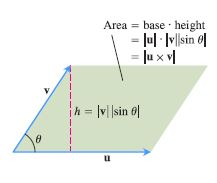
\includegraphics[width=5cm]{week4/calculus}
\end{figure}
For example, suppose that $\bm u=u_1\bm i+u_2\bm j+u_3\bm k,\bm v=v_1\bm i+v_2\bm j+v_3\bm k$. In order to compute the area of the parallelogram determined by $\bm u$ and $\bm v$, we just need to compute the determinant
$\begin{vmatrix}
\bm i&\bm j&\bm k\\u_1&u_2&u_3\\v_1&v_2&v_3
\end{vmatrix}$.
\item
\emph{The product of all the pivots $=(\pm 1)\x$the determinant:}\\
For a 2 by 2 matrix $\bm A=\begin{bmatrix}
a&b\\c&d
\end{bmatrix}$, the pivots are $a$ and $d-(\frac{c}{a})b$. The product of pivots is the determinant:
\[
\text{\emph{Product of pivots}}\qquad a(d-\frac{c}{a}b)=ad-bc\qquad\text{\emph{which is}}\quad \text{det }\bm A
\]
\item
\emph{Compute determinants to find $\bm A^{-1}$ and $\bm A^{-1}\bm b$} (This formula is called \emph{Cramer's Rule}.)
\end{itemize}
\subsubsection{The properties of the Determinant}
We don't intend to define the determinant by its formulas. It's better to start with its properties. These properties are simple, but they prepare for the formulas.
\begin{remark}
Brackets for the matrix, straight bars for its determinant. For example,
\[
\text{The determinant of }\begin{bmatrix}
a&b\\c&d
\end{bmatrix} \text{ is } \begin{vmatrix}
a&b\\c&d\end{vmatrix}=ad-bc
\]
The determinant is written in two ways, det $\bm A$ and $|\bm A|$.
\end{remark}
We will introduce three basic properties, then we will show how properties $1-3$ derive other properties.\\

\begin{enumerate}
\item
\emph{The determinant of the $\bm n$ by $\bm n$ identity matrix is 1.}
\begin{gather*}
\begin{vmatrix}1&0\\0&1\end{vmatrix}=1\qquad\text{and}\qquad\begin{vmatrix}
1&&\\&\ddots&\\&&1\end{vmatrix}=1.
\end{gather*}
\item
\emph{The determianant changes sign when two rows are exchanged.} (sign reversal)
\begin{gather*}
\text{Check:   }\begin{vmatrix}c&d\\a&b\end{vmatrix}=-\begin{vmatrix}a&b\\c&d\end{vmatrix}\qquad\text{(both sides equal $bc-ad$)}.
\end{gather*}
\item
\emph{The determinant is a linear function of each row separately.} (all other rows stay fixed).
\begin{gather*}
\text{\emph{multiply row 1 by any number $\bm t$}}\qquad\begin{vmatrix}ta&tb\\c&d\end{vmatrix}=t\begin{vmatrix}a&b\\c&d\end{vmatrix}
\end{gather*}
\begin{gather*}
\text{\emph{Add row 1 of $\bm A$ to row 1 of $\bm B$:}}\qquad\begin{vmatrix}a_1+a_2&b_1+b_2\\c&d\end{vmatrix}=\begin{vmatrix}a_1&b_1\\c&d\end{vmatrix}+\begin{vmatrix}a_2&b_2\\c&d\end{vmatrix}
\end{gather*}
Note that this rule \emph{deos not} mean $\det (\bm A+\bm B)=\det \bm A+\det\bm B$.\\ Note that this rule \emph{does not} mean $\det(t\bm A)=t\det(\bm A)$. \\Actually, $\det(t\bm A)=t^n\det \bm A$. This is reasonable. Imagining that expanding a rectangle by 2, its area will increase by 4. Expand an $n-$dimensional box by $t$ and its volumn will increase by $t^n$.\\
Pay special attention to property $1-3$. They completely determine the $\det\bm A$. We could stop here to find a formula for determinants. But we prefer to derive other properties that follow directly from the first three.
\item
\emph{If two rows of $\bm A$ are equal, then $\det\bm A=\bm0$.}
\begin{gather*}
\text{Check 2 by 2:   }\begin{vmatrix}a&b\\a&b\end{vmatrix}
=0.
\end{gather*}
Property 4 follows from Property 2.
\begin{proof}[Proofoutline.]
\textit{Exchange the two equal row.} The determinant $\bm D$ is supposed to change sign. But also the matrix is not changed, so we have $-\bm D=\bm D\implies\bm D=0$.
\end{proof}
\item
\emph{Adding a constant multiple of a row to another row doesn't change $\det\bm A$.}
\[
\begin{vmatrix}a+lc&b+ld\\c&d\end{vmatrix}=
\begin{vmatrix}a&b\\c&d\end{vmatrix}+\begin{vmatrix}lc&ld\\c&d\end{vmatrix}=\begin{vmatrix}a&b\\c&d\end{vmatrix}+l\begin{vmatrix}c&d\\c&d\end{vmatrix}=
\begin{vmatrix}a&b\\c&d\end{vmatrix}=\det\bm A
\]
\emph{Conclusion }\textit{The determinant is not changed by the usual elimination step from $\bm A$ to $\bm U$}. Since every row exchange reverses the sign, we have $\det\bm A=\pm\det\bm U$.
\newpage
\item
\emph{If $\bm A$ is triangular, then $\det\bm A=$ product of diagonal entries}.
\begin{gather*}
\text{\emph{Triangular}}\qquad\begin{vmatrix}a&b\\0&d\end{vmatrix}=ad\qquad\text{and also}\qquad\begin{vmatrix}a&0\\c&d\end{vmatrix}=ad
\end{gather*}
Suppose all diagonal entries of $\bm A$ are nonzero. We do Gaussian Elimination to convert $\bm A$ into diagonal matrix:
\[
\det\begin{bmatrix}
a_{11}&&&\bigzero\\&a_{22}&&\\&&\ddots&\\\bigzero&&&a_{nn}
\end{bmatrix}=a_{11}a_{22}\dots a_{nn}.
\]
Factor $a_{11}$ from the first row by property 3; then factor $a_{22}$ from the second row;$\dots\dots$. Finally the determinant is $a_{11}\x a_{22}\x a_{33}\dots\x a_{nn}\x\det\bm I=a_{11}\x a_{22}\x a_{33}\dots\x a_{nn}$.
\item 
$\det(\bm{AB})=\det(\bm A)\det(\bm B)$.
\begin{proof}\qquad\\
\begin{itemize}
\item
If $|\bm B|$ is zero, it's easy to verify that $\bm B$ is singular, then $\bm{AB}$ is singular. Thus $\det(\bm{AB})=0=\det(\bm A)\det(\bm B)$.
\item
Suppose $|\bm B|$ is not zero, and $\bm A,\bm B$ is $n\x n$ matrix. Consider the ratio $D(\bm A)=\frac{|\bm{AB}|}{|\bm B|}$. \textit{Check that this ratio has properties 1,2,3.} If so, $D(\bm A)$ has to be the determinant, say, $|\bm A|$. Thus we have $|\bm A|=\frac{|\bm{AB}|}{\bm B}$:\\\\
\emph{Property 1  }\textit{(Determinant of I)}\quad If $\bm A=\bm I$, then the ratio becomes $D(\bm A)=\frac{|\bm B|}{|\bm B|}=1.$\\\\
\emph{Property 2  }\textit{(Sign reversal)}\quad When two rows of $\bm A$ are exchanged, the same two rows of $\bm{AB}$ are also exchanged. Therefore $|\bm{AB}|$ changes sign and so does the ratio $\frac{|\bm{AB}|}{\bm B}$.\\\\
\emph{Property 3  }\textit{(Linearity)}\quad When row 1 of $\bm A$ is multiplied by $t$, so is row 1 of $\bm{AB}$. Thus the ratio is also increased by $t$. Thus we still have $|\bm A|=\frac{|\bm{AB}|}{\bm B}$.\\
If we Add row 1 of $\bm A_1$ to row 1 of $\bm A_2$. Then row 1 of $\bm A_1\bm B$ also adds to row 1 of $A_2B$. By property three, determinants add. After dividing by $|\bm B|$, the ratios add. Hence we still have $|\bm A|=\frac{|\bm{AB}|}{\bm B}$.\\\\
\textit{Conclusion}\qquad The ratio $D(\bm A)$ has the same three properties that defines determinant, hence it equals $|\bm A|$. Hence we obtain the product rule $|\bm{AB}|=|\bm A||\bm B|$.\\
\end{itemize}
\end{proof}

Immediately here follows a corollary:
\begin{corollary}
\[\det(\bm A^{-1})=\frac{1}{\det(\bm A)}\]
\end{corollary}
\item
\emph{The transpose $\bm A\trans$ has the same determinant as $\bm A$.}
\begin{gather*}
\text{\emph{Transpose}}\qquad\begin{vmatrix}a&b\\c&d\end{vmatrix}=\begin{vmatrix}a&c\\b&d\end{vmatrix}\qquad\text{Both sides equal $ad-bc$}.
\end{gather*}
\begin{proof}
\begin{itemize}
\item
When $\bm A$ is singular, $\bm A\trans$ is also singular. Hence $|\bm A\trans|=|\bm A|=0$.
\item
Otherwise $\bm A$ has LU decomposition $\bm{PA}=\bm{LU}$. Transposing both siders gives $\bm A\trans\bm P\trans=\bm U\trans\bm L\trans$. By product rule we have
\[
\det\bm P\det\bm A=\det\bm L\det\bm U\qquad\text{and}\qquad\det\bm A\trans\det\bm P\trans=\det\bm U\trans\det\bm L\trans.
\]
\begin{itemize}
\item
Firstly, $\det\bm L=\det\bm L\trans=1$. (By property 6, they both have 1's on the diagonal).
\item
Secondly, $\det\bm U=\det\bm U\trans$. (By property 6, they have the same diagonal)
\item
Thirdly, $\det\bm P=\det\bm P\trans$. (Verify by yourself that $\bm P\trans\bm P=\bm I$. Hence $|\bm P\trans||\bm P|=1$. Since permutation matrix is obtained by exchanging rows of $\bm I$, the only possible value for determinant of permuation matrix is $\pm 1$. Hence $\bm P$ and $\bm P\trans$ must both equal to 1 or both equal to -1).
\end{itemize}
So $\bm{L,U,P}$ has the same determinants as $\bm L\trans,\bm U\trans,\bm P\trans$, Hence we have $\det\bm A=\det\bm A\trans$.
\end{itemize}
\end{proof}
\end{enumerate}












